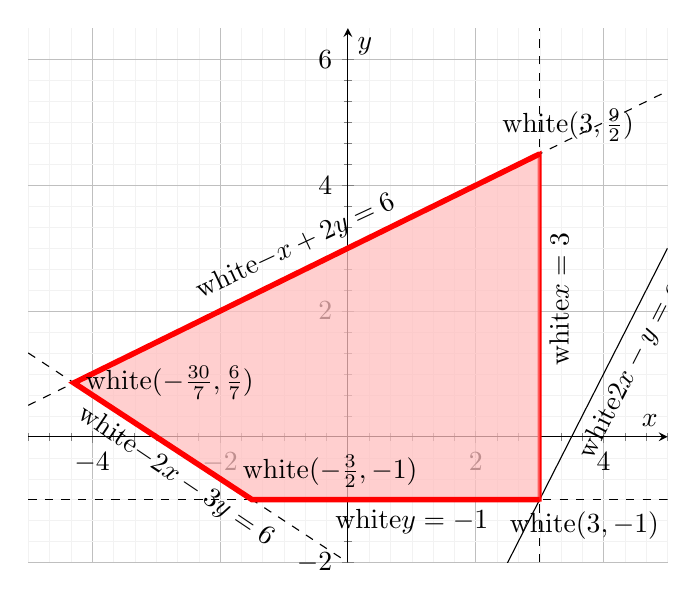
\begin{tikzpicture}
\begin{axis}[
	width=0.8\textwidth,
	axis lines = center,
	xlabel = $x$, ylabel = $y$,
	xmin=-5, xmax=5,
	ymin=-2, ymax=6.5,
	grid=both,
	grid style={line width=.1pt, draw=gray!10},
	major grid style={line width=.2pt,draw=gray!50},
	minor tick num=5,
]

\addplot[
	domain=2:5,
] {2*x-7}
node[pos=0.7, below, rotate=63] {\contour{white}{$2x-y=c$}};

\addplot[
	domain=-5:5,
	dashed,
] {-1}
node[pos=0.6, below] {\contour{white}{$y=-1$}};

\addplot[
	domain=-5:0,
	dashed,
] {-2*x/3-2}
node[pos=0.5, below, rotate=-34] {\contour{white}{$-2x-3y=6$}};

\addplot[
	domain=-5:5,
	dashed,
] {x/2+3}
node[pos=0.6, above left, rotate=25] {\contour{white}{$-x+2y=6$}};

\addplot[
	dashed,
] coordinates {(3, -2) (3, 6.5)}
node[pos=0.35, below right, rotate=90] {\contour{white}{$x=3$}};


\addplot[
	line width=1.5pt,
	color=red,
	fill=pink,
	fill opacity=0.5,
] table {
3 -1
-1.5 -1
-4.286 0.857
3 4.5
} --cycle;

\addplot[
	draw,
	color=red,
	fill=pink,
	fill opacity=0.5,
	line width=2pt,
	point meta=explicit symbolic,
	visualization depends on=\thisrow{align} \as \alignment,
	nodes near coords={
		% add the contour command to the `nodes near coords' output
		% (change the color to see what really is happening)
		\contour{white}{\pgfplotspointmeta}
	},
	node near coords style={
		anchor=\alignment,
		color=black,
		fill opacity=1,
	},
] table[meta index=3] {
	x		y		align		label
	3		-1		150		{$(3, -1)$}
	-1.5		-1		200		{$(-\frac{3}{2}, -1)$}
	-4.286	0.857		180		{$(-\frac{30}{7}, \frac{6}{7})$}
	3		4.5		225		{$(3, \frac{9}{2})$}
};

\end{axis}
\end{tikzpicture}